\documentclass{jaee}


\jlreqsetup{
  thebibliography_indent=0pt
}

\usepackage{tabularray}
\usepackage{url}

\title{日本地震工学会--年次大会講演論文(和文)フォーマット}

\author{佐藤太郎$^{1)}$,鈴木義男$^{2)}$,石川順太$^{3)}$}

\shozoku{
  \begin{tblr}{c}
    1) 正会員\ 東西建設技術研究所,室長\ 博士(工学)\\
    E-mail: sato-t@tozai-tri.co.jp \\
    2) 正会員\ 南大沢大学工学部建築学科,教授\ 工博 \\
    E-mail: yoshios@mou.ac.jp \\
    3) 朱雀市庁,主幹 \\
  \end{tblr}
}

\abstract{本文は\textcolor{red}{日本地震工学会の年次大会}に投稿する際に必要
  となる書式や遵守事項をまとめたサンプル文書である.論文などは以下に記す書
  式に従ってワード・プロセッサなどにより作成する.投稿する際にはAdobe
  Acrobatを用いてPDF形式のファイルに変換し,\textcolor{red}{2〜10ページで容
    量が10 MB未満}になるようにする.投稿先
  は
  \textcolor{red}{\url{http://www.jaee.gr.jp/jp/event/annual/}}
  の論文投稿サイトである.
  ○○○○○○○○○○○○○○○○○○○○○○○○○○○○○○○○○○○○○○○○○○○○○○○○○○○○○○○○○○○○○○○○○○○○○○○}

\keywords{地震,工学,鉄筋コンクリート,せん断}

\begin{document}
\maketitle

\urlstyle{same}
\renewcommand{\thefootnote}{\arabic{footnote}}

\section{用紙のサイズ,余白など}
\label{sec:1}

用紙サイズはA4判として,上の余白は25 mm,下の余白を35 mm,左右の余白を25
mmとする.ただし,1枚めだけは,ヘッダを設ける関係から上部余白を40 mmとする.
1段組に設定して,46字×45行(多少の前後は認める)に設定する.なお,要約部
分およびキーワードの左右の余白は35 mmとする.

1枚めの用紙上端から25 mmの枠外において,左上に本会のロゴマーク(論文等受付
シートに貼付したもの)を貼り付ける.

欄外下部中央(下縁から17 mm)にはページ番号を割り振る.

見本を参考にして,題名,著者名,所属,要約,キーワード,本文,参考文献の順
に作製する.

\section{題目}
\label{sec:2}

論文タイトルは14 ptのゴシック体を用いて中央に印字する.

\section{著者名および所属}
\label{sec:3}

題目から2行の空白のあとに,著者名を14 ptの明朝体で中央に記入する.著者名の
下に1行空白を設けてから,所属を中央に記入する.会員の場合には,会員種別を
最初に記入する.電子メール・アドレスを所有する場合には必ず記入する.和文
は10 ptの明朝体で,英数字は10 ptのTimes New Roman体で記述する.

\section{要約とキーワード}
\label{sec:4}

所属の下に3行の空白をおいて要約を\textcolor{red}{250文字以内}で記述する.な
お「要約」は10 ptのゴシック体で中央に印字し,要約本文は10 ptの明朝体で記述
する.

要約の下に1行の空白をおいてキーワードを10 ptの明朝体で左寄せで記述する.

なお,要約中において既往の研究について文献をあげて述べたい場合には,後述の
本文中で用いる右上添字の文献番号は利用できないので,著者と発刊年を用いる.
(例:「本研究ではPaulay (1976)の手法を拡張する.」)

\section{本文と見出しなど}
\label{sec:5}\vspace{-\baselineskip}

\subsection{本文}
\label{sec:5-1}

キーワードから2行の空白をおいて,本文をはじめる.フォントについては,和文
は10 ptの明朝体で,英数字は10 ptのTimes New Roman体で記述する.章の見出し
は10 ptのゴシック体として,1行空けて本文を続ける.章の見出しのピリオドは半
角「.」で,半角の空白のあとに見出しを続ける.本文の句読点は全角の「,」と
「.」で統一する.段落設定は両端揃えの配置とする.

\subsection{節の小見出しなど}
\label{sec:5-2}

節の小見出しも10 ptのゴシック体として,改行してすぐに本文を続ける.各パラグ
ラフの先頭は1字下げて始め,パラグラフ間には空白を設けない.節の見出しのピ
リオドは半角「.」で,半角の空白のあとに見出しを続ける.

\subsubsection{項の小見出しなど}
\label{sec:5-2-1}

項の小見出しも10 ptのゴシック体として,改行してすぐに本文を続ける.項の間に
は空行は設けない.

\subsubsection{項の小見出しなど}
\label{sec:5-2-2}

項の見出しのピリオドは半角「.」で,半角の空白のあとに見出しを続ける.

\section{数式}
\label{sec:6}

数式は中央に印字し,式番号は(1),(2),として式の最後に右寄せして記す.なお
式の上下には1行ずつの空白を設ける.本文中で式を引用する場合は
式(\ref{eq:1})のようにする.\vspace{-0.7\baselineskip}

\begin{equation}
  V_u = P_w \sigma_{wy}bj\cot{}\phi + bD(1-\beta)\nu_0\sigma_B\tan\theta{}^{*}
  \label{eq:1}
\end{equation}\vspace{-1.5\baselineskip}

\section{図・写真・表・脚注}
\label{sec:7}

図・写真の番号,タイトルはその直下に,表の番号,タイトルはその直上に,それ
ぞれ10 ptのゴシック体で記入する.図・写真および表の呼称は図1,写真1,表1,
のようにして,論文全体を通して番号を振り付ける.なお図,写真および表の左右
には,原則として文字を流し込まない.図,写真および表は本文から1行空けたあと
に貼付する.

図・写真はカラー表示とすることを認める.

脚注\footnote{脚注が必要な場合には引用ページの直近に,左端から5.0 cm程
  度,0.5 pt幅の線を引いた下に,2行程度の範囲で10 ptの明朝体で記述する.}を
入れる場合の書式は,ここに示すとおりである.

\begin{table}
  \centering
  \caption{観測地震動}
  \label{tab:1}
  \begin{tblr}{hlines,
    vlines,
    cells={c},
    rowsep=0pt}
      % {|c|c|c|c|c|c|c|}
    \SetCell[r=3,c=1]{c} 日付
    & \SetCell[r=3,c=1]{c} 時刻
    & \SetCell[r=1,c=3]{c} 1F &&
    & \SetCell[r=1,c=2]{c} 5F & \\
    & & {計測震度\\相当値}
    & \SetCell[r=1,c=2]{c} {最大加速度\\(m/s$^2$)} &
    & \SetCell[r=1,c=2]{c} {最大加速度\\(m/s$^2$)} & \\\cline{4-7}
    & & {\footnotesize (水平2方向\\による)}
    & {N/S\\(梁間)} & {E/W\\(桁行)}
    & {N/S\\(梁間)} & {E/W\\(桁行)} \\\hline
    \SetCell[r=3]{h}10/23 & 17:56 & 4.4 & 0.72 & 1.07 & 1.78 & 3.26 \\
    & 18:03 & 3.1 & 0.23 & 0.27 & 0.51 & 0.68 \\
    & 18:12 & 3.1 & 0.12 & 0.25 & 0.43 & 0.70
  \end{tblr}
\end{table}

\begin{figure}
  \centering
  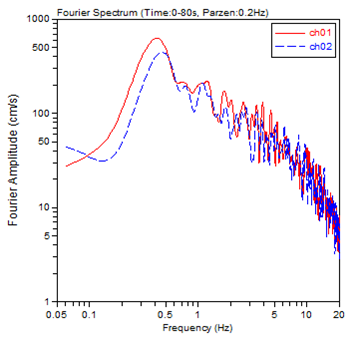
\includegraphics[height=89mm]{fig1}
  \caption{観測波のフーリエスペクトル}
  \label{fig:1}
\end{figure}

\section{使用する単位とフォント}
\label{sec:8}

単位は原則としてSI単位系に統一する.提出された論文の書誌情報はxml形式でJ-STAGEに登録される.この際,J-STAGE側で用意してある書誌XML作成ツールを用いて論文(PDFファイル)から書誌情報を自動生成する際の要件として,下記のようなフォントの指定がなされているので,これに従うこと.

\newpage

\begin{table}
  \centering
  \caption{jaee書誌XML作成ツールで指定されているフォント}
  \label{tab:2}
  \begin{tblr}{|Q[c,m]|Q[c,m]|Q[c,m]|}
    \hline
    \SetCell{bg=green} {\mcfamily\bfseries テンプレート名} &
                                                             \SetCell[c=2]{c, bg=green} \textbf{jaee\_basic} \\\hline
    \SetCell{bg=green} テンプレート項目 & \SetCell{bg=green} フォント名 & \SetCell{bg=green} フォントサイズ \\\hline
    記事タイトル(日) & MS Pゴシック & 14.0 \\\hline
    著者(日) & MS 明朝 & 14.0 \\\hline
    所属(日) & MS 明朝 & 10.0 \\\hline
    抄録(日)タイトル & MS ゴシック & 10.0 \\\hline
    抄録(日) & MS 明朝 & 10.0 \\\hline
    キーワード(日) & MS 明朝,斜体 & 10.0 \\\hline
    参考文献 & {(日) MS 明朝\\(英数) Times New Roman} & 10.0 \\\hline
    記事タイトル(英) & Times New Roman, Bold & 14.0 \\\hline
    著者(英) & Times New Roman & 14.0 \\\hline
    所属(英) & Times New Roman & 10.0 \\\hline
    抄録(英) & Times New Roman, Bold & 10.0 \\\hline
    キーワード(英) & Times New Roman, Italic & 10.0 \\\hline
  \end{tblr}
\end{table}

\section{謝辞}
\label{sec:9}

謝辞がある場合には,本文の結論の末尾に和文は10 ptの明朝体で,英数字は10
ptのTimes New Roman体で記述する.

\section{参考文献}
\label{sec:10}

参考文献のリストは,10 ptの明朝体で記述する.参照した順に番号を振って,結論,
謝辞のあとに,記載例に従って記載する.\textcolor{red}{記載方法については,
  日本地震工学会論文集の執筆要領を参照すること.}

本文中での参考文献の表示は,該当箇所に文献番号を右上添字で1),2),・・・と
記す.著者を含めた記載としたい場合には次の例文を参考にされたい.「この研究
はPaulay\cite{bib:1}によって始められた.その後,久保・小原\cite{bib:2},建
築・白川$^{3)}$,高畑ら$^{4)}$,Takeuchi et al.$^{5)}$によって発展し
た.1980年代までの研究成果$^{1), 2)}$ と比較すると,それ以降の研究成
果$^{3)-5)}$では....」\vspace{\baselineskip}

\section*{謝 辞}
\label{sec:shaji}
\vspace{-0.6\baselineskip}

本論の作成に当たっては,関係各位のご協力を得ました.記して御礼申し上げます.

\begin{thebibliography}{99}
\bibitem{bib:1} Pauay, T.: Moment Redistribution in Continuous Beam of
  Earthquake Resistant Multistory Reinforced Concrete Frames, Bulletin of
  New Zealand National Society for Engineering, Vol. 9, No. 4,
  pp.205--212, 1976.
\bibitem{bib:2} 久保哲夫,小原明: RC造骨組みに関する研究, 日本建築学会梗概
  集, Vol. C, pp.719--720, 1987.
\end{thebibliography}

\end{document}
